\subsection{Branchenanalyse} \label{Branchen}
    Um die Situation und Position eines Unternehmens einordnen zu können steht u.a. die Branchenanalyse zur Verfügung.
    Bei der Branchenanalyse werden die Einflussfaktoren auf eine Branche ermittelt und bewertet. Dabei ist eine Branche
    ein Marktsegment mit Produkten, die untereinander substituierbar sind. Die Einflussfaktoren auf die Branche haben
    verschiedene Herkunft und auch unterschiedlich starken Einfluss.

    \noindent
    Das Five-Forces Modell nach Porter beschreibt die Einflussfaktoren, bewertet diese und stellt die Marktattraktivität
    da.

    \noindent
    Die Five-Forces (fünf Kräfte) bestehen aus der Verhandlungsmacht der Lieferanten (Vertragspartner bei denen Produkte
    eingekauft werden), der Verhandlungsmacht der Kunden, Bedrohung durch neue Wettbewerber (Markteintrittsbarrieren),
    Bedrohung durch Ersatzprodukte (Substitute im weiteren Sinne) und der Wettbewerbsintensität der Branche.
    (Vgl. \cite{Gamayanto2005}, S.\,128-129)

    \noindent
    Die Verhandlungsmacht der Lieferanten beschreibt den Einfluss, den die Lieferanten auf das Unternehmen haben. Kann
    auf die Produkte des Lieferanten nicht verzichtet werden, sind z.B. keine Substitute vorhanden, wird das Unternehmen
    abhängiger. Faktoren können die Anzahl der Anbieter, Vertragssicherheit, die Verzichtbarkeit und Substitute sein.

    \noindent
    Die Verhandlungsmacht des Kunden beschreibt den Einfluss der Kunden. Der Einfluss wächst mit zunehmender Anzahl an
    Marktbegleitern und Substituten. Wächst der Kundenkreis schneller als der Anbieterkreis (bei stetiger
    Produktionsmenge) sinkt die Verhandlungsmacht der Kunden. Sind die Umstellungskosten für die Kunden auf ein neues
    Produkt groß (Gewöhnung oder Verbundprodukte) sinkt auch der Einfluss.

    \noindent
    Bedrohung durch neue Wettbewerber. Hier stellt sich die Frage wie schwer es für potenzielle neue Anbieter ist den
    Markt zu betreten. Ist z.B. für die Herstellung eine bestimmte Genehmigung oder Handelspartner notwendig, sinkt das
    Risiko durch neue Wettbewerber. Sind die Einstiegsbarrieren aber niedrig, weil z.B. keine kapitalintensiven
    Investitionen getätigt werden müssen, steigt das Risiko.

    \noindent
    Die Wettbewerbsintensität beschreibt die Gesamtsituation. Desto intensiver ein Wettbewerb ist, desto geringer sind
    die Aussichten auf ein gewinnbringendes Geschäft. Einflüsse wie Anzahl der Wettbewerber, Branchenwachstum,
    Austrittsbarrieren und Produktdifferenzierung spielen hier eine entscheidende Rolle. Anbieter, die keine starken
    Alleinstellungsmerkmale besitzen, können leichter aus der Branche gedrängt werden.

    %todo: Section anpassen
    \noindent
    Five Forces Modell angewandt

    \noindent
    Für die Verhandlungsmacht der Lieferanten wurde beispielhaft die Computer Chip Branche genutzt. Computer Chips
    werden von wenigen Produzenten in großer Stückzahl hergestellt. Dies Produzenten verkaufen große Mengen an
    Großhändler. Da die Menge an Chips pro Gerät vgl. gering ist, können viele Großhändler noch die extra Kapazitäten
    beim Hersteller einkaufen. Somit ist die Wahl des Großhändlers flexibel und der Lieferant hat eine geringe
    Verhandlungsmacht.

    \noindent
    Die Bedrohung durch neue Wettbewerber wird als gering betrachtet. Neue Wettbewerber müssen Kapital in der
    Entwicklung und den Aufbau einer Produktionsstätte binden. Zudem müssen für bestimmte Absatzwege hohe Barrieren
    überwunden werden (z.B. Aufnahme im Einzelhandel).

    \noindent
    Die Verhandlungsmacht der Kunden wird zur Markteinführung als gering eingeschätzt. Es wird davon ausgegangen, dass
    der Verkaufsstart auf einen ungesättigten Markt erfolgreich gelingt und die Nachfrage größer als das Angebot ist.

    \noindent
    Die Reinigung von Dachrinnen ist durch eine Vielzahl von Ersatzprodukten gekennzeichnet. So könnte der Hausbesitzer
    auf einen Dienstleister zurückgreifen oder die Dachrinnen eigenständig von Hand reinigen. Die Gefahr von
    Ersatzprodukten ist besonders im privaten Bereich groß.

    \noindent
    Aus den vier Bereichen kann die Rivalität unter den Wettbewerbern abgeleitet werden. Für die Erfolgsaussichten
    positiv ist die geringe Anzahl an Mitbewerbern, die geringe Macht der Lieferanten und Kunden und hohe
    Markteintrittsbarrieren.

    \noindent
    Negativ für die Erfolgsaussichten ist die Vielzahl an Ersatzprodukte, die finanziell günstiger und verbreiteter
    sind.

    \noindent
    Daraus lässt sich ableiten, dass die Rivalität auf dem Markt nicht sehr hoch ist und das Marktsegment große
    Erfolgsaussichten bieten. Für einen Erfolg sollte sich von Ersatzprodukten abgegrenzt werden.

    \begin{figure}[ht]
        \centering
        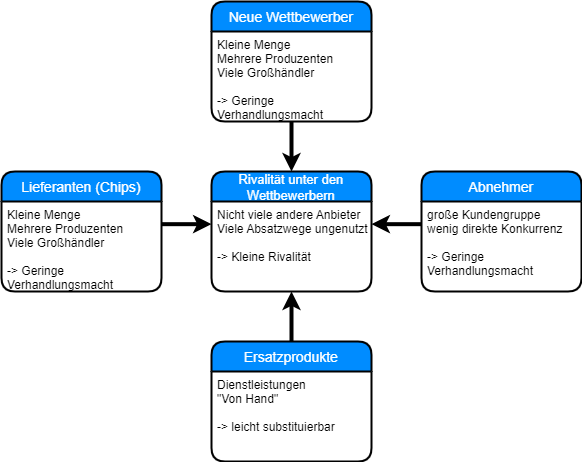
\includegraphics[width = 0.9\textwidth]{Eigene Darstellungen/Distributionswege2.png}

        \caption{Five Forces (Eigene Darstellung, in Anlehnung an \cite{Gamayanto2005}, S.\,127)}
    \end{figure}

